% Chapter 5: Constructions in the Abstract
% DEFINES: ch:constructions-abstract; sec:strategies, sec:acceptance,
%   sec:space-duality, sec:ch5-notes; def:acceptance, prop:space-duality,
%   ex:acceptance-watchlist, ex:space-watchlist, fig:acceptance, rem:lower-bound
% REFERENCES (backward): def:cipher-map, sec:totality-support, ex:watchlist-numbers,
%   def:uniformity, def:correctness, sec:parameter-tuple
% REFERENCES (forward, part labels): part:constructions, part:confidentiality

\chapter{Constructions in the Abstract}
\label{ch:constructions-abstract}

The previous two chapters said what a cipher map \emph{is} and what it must
satisfy. They did not say how to build one. This chapter takes the last step
of the keystone: it describes construction at the level of abstraction where
all the concrete schemes look the same. There are two strategies, batch and
online; there is a single device, the acceptance predicate, that every batch
construction instantiates; and there is one law, the space-accuracy duality,
that fixes what a cipher map must cost. The concrete realizations, the
hash-set, the codec, the algebraic Boolean construction, are
\Cref{part:constructions}; here they are previewed as instances of one
picture.

\section{Two Strategies: Batch and Online}
\label{sec:strategies}

\Cref{sec:three-transformations} distinguished two ways to produce the total
function $\fhat$, and the distinction organizes every construction in the
book. They differ in when the work is done and in what they can compute.

A \emph{batch} construction searches for a secret $s$ that makes $\fhat$
correct on all of $X$ at once. The trusted machine knows the domain $X$ and
the latent function $f$ at build time, and it tries seeds until it finds one
whose induced $\fhat$ lands every in-domain element in the right place, up to
the error budget $\eta$. The cost is paid in construction: the search can be
long, and it grows with how strict the budget is. The reward is a structure
that is near information-theoretically minimal in space and whose error is
tunable by how hard one is willing to search. The watchlist of
\Cref{ex:watchlist-numbers} is naturally a batch construction: with four
names and a target $\eta$, the trusted machine searches for a seed under
which alice, bob, carol, and dave each hash into the codeword region for
their correct answer.

An \emph{online} construction reads $\fhat$ directly off a hash structure
with no search at all. The secret is just a hash key, and the function is
whatever the structure computes algebraically on its inputs. Nothing is
pre-solved, so an online construction pays almost nothing to build, but it
can only compute the operations its structure supports natively, the
trapdoor Boolean algebra of \Cref{part:algebra} being the example, where
set operations are realized as bit operations on hash images. Both
strategies produce objects satisfying \Cref{def:cipher-map}; they sit at
opposite ends of a trade between build cost and expressive freedom, and
\Cref{part:constructions} works each out concretely.\footnote{The hash-set,
the entropy map, and the codec construction (batch), and the algebraic
Boolean construction (online), with their seed searches, space, and error,
are the subject of \Cref{part:constructions}.}

\section{The Acceptance Predicate}
\label{sec:acceptance}

Underneath every batch construction is the same object, and naming it is
what lets one treatment cover schemes that look unrelated. The decoder
$\dec$ sorts tokens by the value they carry; the sets it sorts them into are
the acceptance regions.

\begin{definition}[Acceptance predicate]
\label{def:acceptance}
For a cipher map with decoder $\dec : \B^n \to Y \cup \{\bot\}$ and each
value $y \in Y$, the \emph{acceptance region} is the set of tokens that
decode to $y$,
\[
  A(y) \;=\; \{\, c \in \B^n : \dec(c) = y \,\}.
\]
The regions $\{A(y)\}_{y \in Y}$ are disjoint, their union is the set of
valid codewords, and every remaining token decodes to $\bot$. The
\emph{acceptance probability} of $y$ is $\alpha(y) = \lvert A(y)\rvert / 2^n$,
and the noise-decode probability of \Cref{sec:totality-support} is their sum,
\[
  \varepsilon \;=\; \sum_{y \in Y} \alpha(y)
  \;=\; \frac{\lvert \bigcup_y A(y)\rvert}{2^n}.
\]
\end{definition}

A cipher map, viewed through its decoder, is nothing more than a partition
of the token space into the value regions $\{A(y)\}$ and a noise region that
decodes to nothing (\Cref{fig:acceptance}). To build a batch cipher map is to
choose those regions and then search for a seed that drops each in-domain
element into the region for its correct answer. This is the device that
unifies the constructions. A hash-set is the partition with a single
accept region (a token is in the set or it is noise); a frequency-smoothing
map sizes its regions to the value distribution; an encrypted membership
index is the two-region partition for a Boolean answer. They are one
construction with different choices of $\{A(y)\}$.

\begin{figure}[t]
\centering
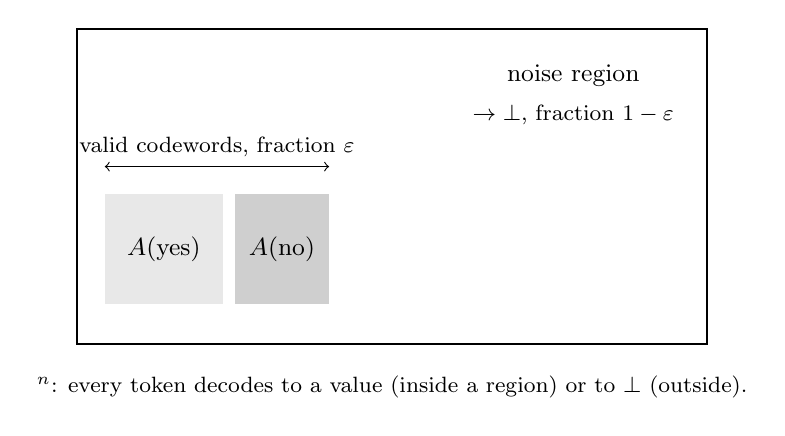
\begin{tikzpicture}[font=\small]
\draw[thick] (0,0) rectangle (8,4);
\node at (6.3,3.4) {noise region};
\node at (6.3,2.9) {\footnotesize $\dec \to \bot$,\ fraction $1-\varepsilon$};
\fill[gray!18] (0.35,0.5) rectangle (1.85,1.9);
\fill[gray!38] (2.0,0.5) rectangle (3.2,1.9);
\node at (1.1,1.2) {$A(\mathrm{yes})$};
\node at (2.6,1.2) {$A(\mathrm{no})$};
\draw[<->] (0.35,2.25) -- (3.2,2.25)
  node[midway,above,align=center]{\footnotesize valid codewords,\ fraction $\varepsilon$};
\node[align=left] at (4.0,-0.55)
  {\footnotesize $\B^n$: every token decodes to a value (inside a region) or to $\bot$ (outside).};
\end{tikzpicture}
\caption{A cipher map as a partition of the token space. The acceptance
regions $\{A(y)\}$ hold the valid codewords (a fraction $\varepsilon$ of
$\B^n$); everything else is noise. A batch construction chooses the regions,
then seeds $\fhat$ so each in-domain element lands in the region for its
answer.}
\label{fig:acceptance}
\end{figure}

The freedom is in the \emph{sizes}. Making $A(y)$ larger makes a value
easier to hit and the structure cheaper, but it raises $\varepsilon$ and so
the noise. The allocation that minimizes the value-encoding cost is the
Shannon-optimal one: size each region in proportion to how often its value
occurs,
\[
  \lvert A(y)\rvert \;\propto\; \Pr[f(X) = y],
\]
so that common answers get large regions and rare answers small ones,
exactly source coding applied to the output distribution. With this
allocation the per-element cost of carrying the value equals the entropy
$H(Y)$, which is the content of the next section.

\begin{example}[The watchlist partition]
\label{ex:acceptance-watchlist}
The membership map has two values, and on the four names with set
$S = \{\mathrm{alice}, \mathrm{carol}\}$ both answers are equally likely,
$\Pr[\text{yes}] = \Pr[\text{no}] = \tfrac12$, so the Shannon allocation
makes the two regions equal, $\lvert A(\mathrm{yes})\rvert =
\lvert A(\mathrm{no})\rvert$. With the $n = 12$ token space of
\Cref{ex:watchlist-numbers} and a target noise floor $\varepsilon \approx
10^{-3}$, the two regions together hold about four of the $4096$ codewords,
two apiece; the other $4092$ strings decode to $\bot$. Building the map is
then the search for a seed under which each member hashes into
$A(\mathrm{yes})$ and each non-member into $A(\mathrm{no})$.
\end{example}

\section{The Space-Accuracy Duality}
\label{sec:space-duality}

The acceptance picture makes the cost of a cipher map legible. A token must
do two things: stand out from noise, and name a value. Each has an
information price, and the two prices add.

\begin{proposition}[Space-accuracy duality]
\label{prop:space-duality}
A cipher map storing $f : X \to Y$ with noise-decode probability
$\varepsilon$ and Shannon-optimal value regions costs, per element,
\[
  \text{bits/element} \;=\; -\log_2 \varepsilon \;+\; \mu,
  \qquad \mu = H(Y),
\]
where $-\log_2 \varepsilon$ is the cost of separating signal from noise and
$\mu = H(Y)$ is the cost of encoding the value.
\end{proposition}

\begin{proof}[Derivation]
Split the per-element cost into the two tasks. To stand out from noise, an
element's codeword must lie in the valid set, which occupies a fraction
$\varepsilon$ of $\B^n$; pinning a token down to a set of relative measure
$\varepsilon$ takes $\log_2(1/\varepsilon) = -\log_2\varepsilon$ bits, the
address of the signal inside the noise. To name the value, observe that the
decoded answer is distributed as $f(X)$, and by Shannon source coding the
average number of bits to encode a draw from that distribution is its
entropy $H(Y)$, achieved exactly when the regions are sized
$\lvert A(y)\rvert \propto \Pr[f(X) = y]$ as in \Cref{sec:acceptance}. The
two costs are over independent descriptions, the location of the codeword
and its label, so they add: $-\log_2\varepsilon + H(Y)$.
\end{proof}

The duality says where a cipher map's space goes, and the two terms answer
to different parameters of \Cref{sec:parameter-tuple}. The first term,
$-\log_2\varepsilon$, is the price of hiding: a smaller $\varepsilon$ buries
the signal in more noise, raising confidentiality at a logarithmic cost in
bits. The second, $\mu = H(Y)$, is the price of the answer and is
irreducible: no construction encodes the values in fewer than $H(Y)$ bits on
average. Correctness $\eta$ sits orthogonal to both; it trades against
construction time, not space.

\begin{example}[Bits for the watchlist]
\label{ex:space-watchlist}
The watchlist is a Boolean map with balanced answers, so $\mu = H(Y) = 1$
bit. At the noise floor $\varepsilon \approx 10^{-3}$ of
\Cref{ex:acceptance-watchlist}, the hiding term is $-\log_2 10^{-3} =
\log_2 1000 \approx 9.97$ bits, so the map costs about $9.97 + 1 \approx 11$
bits per name. Almost all of it pays to hide the answer in noise; a single
bit carries the membership fact itself. Tightening $\varepsilon$ to
$10^{-6}$ would roughly double the hiding term to $\approx 20$ bits while
leaving the value bit untouched, the logarithmic price of an extra factor of
a thousand in noise.
\end{example}

\begin{remark}[Optimality]
\label{rem:lower-bound}
The duality is not merely an accounting of one construction; it is a floor.
No cipher map for $f$ can use fewer than $-\log_2\varepsilon + H(Y)$ bits per
element on average: the value term is forced by source coding, and the noise
term is forced because a structure smaller than $-\log_2\varepsilon$ bits
would leave the valid codewords denser than a fraction $\varepsilon$ and so
admit more than the allotted noise. The matching bound, that the
hash-based construction achieves this floor, is established in the
Bernoulli entropy analysis and restated in the cipher-maps
paper.\footnote{The tight lower bound and its achievability are proved in the
companion work \cite{towell2026cipher}; the monograph states the result and
points there rather than reproducing the proof.}
\end{remark}

\section{Notes and Provenance}
\label{sec:ch5-notes}

The batch and online strategies and the acceptance predicate are the
cipher-maps paper's; the spine names the acceptance partition $\{A(y)\}$ with
$\alpha(y) = \lvert A(y)\rvert/2^n$ and $\varepsilon = \sum_y \alpha(y)$, and
this chapter follows it. The space-accuracy duality $-\log_2\varepsilon +
H(Y)$ has three independent derivations across the two ecosystems, the
Bernoulli entropy lower bound, the entropy-map construction, and the
hash-function space analysis, which converge on the same two terms; the book
takes the duality as the abstract law and defers the tight lower bound and
its achievability to \Cref{part:constructions} and the companion paper. The
acceptance partition returns in \Cref{part:confidentiality}, where the
\emph{shape} of the regions controls confidentiality, and the surprise is
that there is no single best shape. The allocation that is space-optimal
here, sized to the value distribution, is not the one that flattens token
frequency, and neither is the one that best resists a multi-instance
adversary aligning independent cipher maps for the same function; the three
pull in different directions, a frontier rather than an optimum, which
\Cref{part:confidentiality} and \Cref{ch:gf2-retrieval} develop. With this chapter the keystone is complete: the cipher map is
defined, its four properties are fixed with their parameters, and its
abstract construction and cost are in hand, enough for the algebra of
\Cref{part:algebra} to build on.
